\documentclass[10pt, aspectratio=169]{beamer}
\usepackage[utf8]{inputenc}
\usepackage[T1]{fontenc}
\usepackage{amsmath, amsfonts, amssymb, amsthm}
\usepackage{booktabs}
\usepackage{graphicx}
\usepackage{tikz}
\usetikzlibrary{shapes.geometric, arrows, positioning, fit, backgrounds}

% Theme selection
\usetheme{metropolis} 
\usecolortheme{default}

\title{Metodologi Penelitian: Implementasi qPCA pada Model Heath-Jarrow-Morton (HJM)}
\subtitle{Studi Kasus: Phys. Rev. Research 3, 013167 (2021)}
\author{Review Project}
\date{\today}

\begin{document}

\maketitle

\begin{frame}{Outline Metodologi}
    \tableofcontents
\end{frame}

\section{Akuisisi Data dan Pre-processing}
\begin{frame}{1. Akuisisi Data dan Pre-processing}
    \begin{itemize}
        \item \textbf{Pengambilan Data:} Data historis \textit{forward rates} diekstraksi untuk tenor \textit{1, 3, dan 6 bulan} guna membangun struktur stokastik model HJM.
        \item \textbf{Konstruksi Matriks Kovarians:} Menghitung korelasi silang dari perubahan \textit{forward rates}. Contoh matriks $\sigma_3$ (unit $10^{-4}$):
        \begin{equation}
            \sigma_3 = \begin{pmatrix} 1.89 & 0.97 & 0.91 \\ 0.97 & 1.06 & 1.01 \\ 0.91 & 1.01 & 1.26 \end{pmatrix}
        \end{equation}
        \item \textbf{Normalisasi Matriks Densitas:} Transformasi matriks menjadi $\rho$ dengan syarat $\text{tr}[\rho] = 1$ untuk pemetaan ke dalam sistem kuantum.
        \item Untuk sub-kasus $2 \times 2$ (maturitas 1 dan 3 bulan):
        \begin{equation}
            \rho_2 = \begin{pmatrix} 0.6407 & 0.3288 \\ 0.3288 & 0.3593 \end{pmatrix}
        \end{equation}
    \end{itemize}
\end{frame}


\section{Strategi Reduksi Dimensi (PCA)}
\begin{frame}{2. Strategi Reduksi Dimensi (PCA)}
    \begin{itemize}
        \item \textbf{Analisis Spektral:} Identifikasi \textit{eigenvalue} dominan pada $\rho_2$ untuk menyederhanakan kompleksitas:
        \begin{equation}
            \lambda_1 = 0.8576, \quad \lambda_2 = 0.1424
        \end{equation}
        \item \textbf{Vektor Eigen:} Menentukan profil volatilitas utama (\textit{parallel shift} dan \textit{twist}):
        \begin{align}
            |u_1\rangle &= 0.8347|0\rangle + 0.5508|1\rangle \\
            |u_2\rangle &= 0.5508|0\rangle - 0.8347|1\rangle
        \end{align}
        \item \textbf{Reduksi Faktor Noisy:} Mengingat $\lambda_{max} \gg \lambda_2$, model direduksi menjadi \textit{low-rank} untuk meminimalkan jumlah gerbang (\textit{gates}) dan mempertahankan koherensi qubit pada era NISQ.
    \end{itemize}
\end{frame}


\section{Desain Sirkuit dan Algoritma Kuantum (qPCA)}
\begin{frame}{3. Desain Sirkuit dan Algoritma Kuantum (qPCA)}
    \begin{itemize}
        \item \textbf{Evolusi Uniter:} Implementasi operator $U = e^{2\pi i \rho}$ pada prosesor \textbf{IBMQX2 5-qubit}.
        \item Matriks uniter untuk kasus $2 \times 2$:
        \begin{equation}
            U_{\rho_2} = \begin{pmatrix} 0.6260 - 0.3068i & -0.7170i \\ -0.7170i & 0.6260 + 0.3068i \end{pmatrix}
        \end{equation}
        \item \textbf{Alokasi Sumber Daya:}
        \begin{itemize}
            \item \textbf{Register Nilai Eigen:} Menggunakan $n=2$ atau $n=3$ qubit.
            \item \textbf{Register Vektor Eigen:} Menggunakan 1--2 qubit penyandian.
        \end{itemize}
        \item \textbf{Eksekusi:} Setiap sirkuit dijalankan dengan \textit{8192 realizations (shots)} untuk mitigasi galat statistik.
    \end{itemize}
\end{frame}


\section{Protokol Eksperimental Iteratif}
\begin{frame}{4. Protokol Eksperimental Iteratif}
    \begin{itemize}
        \item \textbf{Tahap I: Estimasi Vektor Eigen:} Dimulai dari \textit{random state} $|b_0\rangle$, diproyeksikan pada estimasi biner 2-bit ($\Lambda_{max} = 0.11$).
        \item Konvergensi tercapai pada iterasi ke-4:
        \begin{equation}
            |u_{max}\rangle_{2\times2} = [(0.87 \pm \delta) - i(0.10 \pm \delta)]|0\rangle + [(0.47 \pm \delta) + i(0.10 \pm \delta)]|1\rangle
        \end{equation}
        \item \textbf{Tahap II: Perbaikan Nilai Eigen:} Menggunakan $|u_{max}\rangle$ sebagai input QPE 3-bit pada simulator QISKIT.
        \item Hasil menunjukkan $\Lambda = 0.111$ (desimal 0.875) dengan \textit{Fidelity} 0.965 terhadap nilai eksak.
    \end{itemize}
\end{frame}


\section{Mitigasi Galat dan Skalabilitas}
\begin{frame}{5. Mitigasi Galat dan Skalabilitas}
    \begin{itemize}
        \item \textbf{Error Mitigation:} Menggunakan \textit{Richardson's extrapolation} dan rotasi basis untuk menangani \textit{Gate Error} (8\%/gate) dan \textit{Statistical Error} (11\%).
        \item \textbf{Kasus $4 \times 4$:} Meskipun terjadi akumulasi galat signifikan pada hardware ($>100\%$ pada 18 gerbang), dekomposisi teoretis tetap konsisten dengan $\lambda_4 = 0.800$.
        \item \textbf{Hasil Simulator $4 \times 4$:}
        \begin{multline}
            |u_{max}\rangle = (0.6287 + i0.3991)|00\rangle + (0.4010 + i0.0693i)|01\rangle \\
            + (0.4807 - i0.1964)|10\rangle + (0.0305 + i0.0959)|11\rangle
        \end{multline}
    \end{itemize}
\end{frame}


\section{Diagram Alir Metodologi}
\begin{frame}{6. Diagram Alir Metodologi (1/2)}
    \centering
    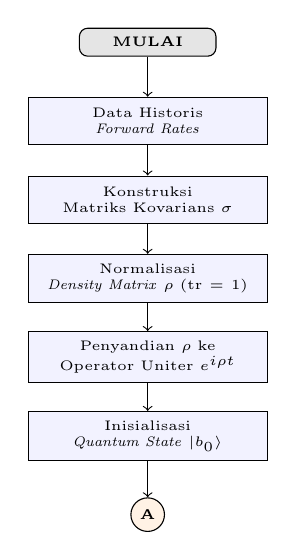
\begin{tikzpicture}[
        node distance=1.0cm,
        every node/.style={fill=white, font=\tiny, align=center},
        block/.style={rectangle, draw, text width=2.8cm, minimum height=0.6cm, fill=blue!5},
        terminal/.style={rectangle, draw, rounded corners=3pt, text width=1.5cm, fill=gray!20, font=\tiny\bfseries},
        connector/.style={circle, draw, fill=orange!10, inner sep=2pt, font=\tiny\bfseries}
    ]
        % Terminals & Pre-processing
        \node (mulai) [terminal] {MULAI};
        \node (start) [block, below of=mulai] {Data Historis \\ \textit{Forward Rates}};
        \node (matriks) [block, below of=start] {Konstruksi \\ Matriks Kovarians $\sigma$};
        \node (norm) [block, below of=matriks] {Normalisasi \\ \textit{Density Matrix} $\rho$ ($\text{tr}=1$)};
        \node (uniter) [block, below of=norm] {Penyandian $\rho$ ke \\ Operator Uniter $e^{i\rho t}$};
        \node (init) [block, below of=uniter] {Inisialisasi \\ \textit{Quantum State} $|b_0\rangle$};
        
        % Terminal Connector A
        \node (connA) [connector, below of=init] {A};

        % Connections
        \draw [->] (mulai) -- (start);
        \draw [->] (start) -- (matriks);
        \draw [->] (matriks) -- (norm);
        \draw [->] (norm) -- (uniter);
        \draw [->] (uniter) -- (init);
        \draw [->] (init) -- (connA);
    \end{tikzpicture}
\end{frame}

\begin{frame}{6. Diagram Alir Metodologi (2/2)}
    \centering
    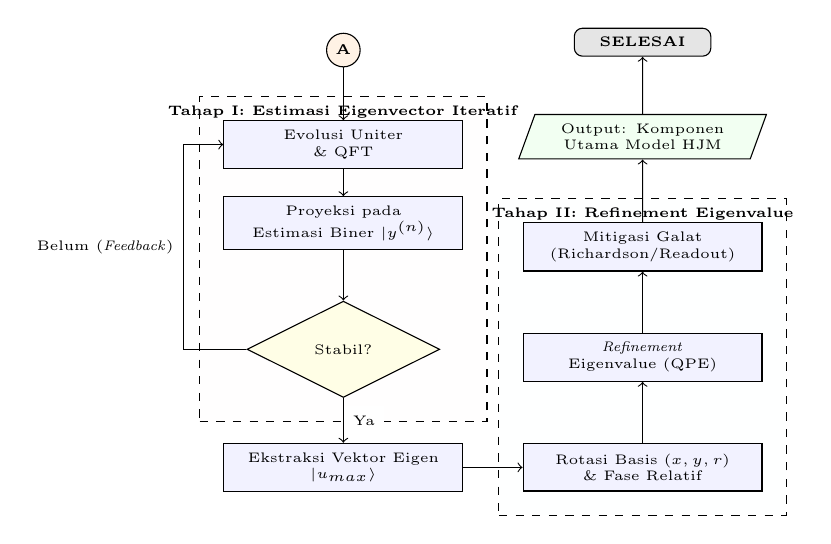
\begin{tikzpicture}[
        node distance=1.0cm,
        every node/.style={fill=white, font=\tiny, align=center},
        block/.style={rectangle, draw, text width=2.8cm, minimum height=0.6cm, fill=blue!5},
        decision/.style={diamond, draw, aspect=2, text width=1.5cm, fill=yellow!10},
        io/.style={trapezium, trapezium left angle=70, trapezium right angle=110, draw, fill=green!5, text width=2.5cm},
        terminal/.style={rectangle, draw, rounded corners=3pt, text width=1.5cm, fill=gray!20, font=\tiny\bfseries},
        subgraphI/.style={draw, dashed, inner sep=0.3cm, fill=red!5, fill opacity=0.1},
        subgraphII/.style={draw, dashed, inner sep=0.3cm, fill=cyan!5, fill opacity=0.1},
        connector/.style={circle, draw, fill=orange!10, inner sep=2pt, font=\tiny\bfseries}
    ]
        % Entry Connector A
        \node (connA) [connector] {A};
        
        % Tahap I: Iterative Eigenvector Estimation
        \node (evolusi) [block, below of=connA, node distance=1.2cm] {Evolusi Uniter \\ \& QFT};
        \node (proyeksi) [block, below of=evolusi] {Proyeksi pada \\ Estimasi Biner $|y^{(n)}\rangle$};
        \node (stabil) [decision, below of=proyeksi, node distance=1.6cm] {Stabil?};
        \node (isolasi) [block, below of=stabil, node distance=1.5cm] {Ekstraksi Vektor Eigen \\ $|u_{max}\rangle$};

        % Tahap II: Eigenvalue Refinement
        \node (fase) [block, right of=isolasi, node distance=3.8cm] {Rotasi Basis ($x, y, r$) \\ \& Fase Relatif};
        \node (refine) [block, above of=fase, node distance=1.4cm] {\textit{Refinement} \\ Eigenvalue (QPE)};
        \node (mitigasi) [block, above of=refine, node distance=1.4cm] {Mitigasi Galat \\ (Richardson/Readout)};
        
        % Output & Terminal
        \node (result) [io, above of=mitigasi, node distance=1.4cm] {Output: Komponen \\ Utama Model HJM};
        \node (selesai) [terminal, above of=result, node distance=1.2cm] {SELESAI};

        % Connections
        \draw [->] (connA) -- (evolusi);
        \draw [->] (evolusi) -- (proyeksi);
        \draw [->] (proyeksi) -- (stabil);
        \draw [->] (stabil) -- node[anchor=west] {Ya} (isolasi);
        \draw [->] (stabil.west) -- ++(-0.8,0) |- node[anchor=east, pos=0.25] {Belum (\textit{Feedback})} (evolusi.west);
        \draw [->] (isolasi) -- (fase);
        \draw [->] (fase) -- (refine);
        \draw [->] (refine) -- (mitigasi);
        \draw [->] (mitigasi) -- (result);
        \draw [->] (result) -- (selesai);

        % Subgraph Boxes
        \begin{pgfonlayer}{background}
            \node [subgraphI, fit=(evolusi) (proyeksi) (stabil), label={[shift={(0,-0.4)}]above:\textbf{Tahap I: Estimasi Eigenvector Iteratif}}] {};
            \node [subgraphII, fit=(fase) (refine) (mitigasi), label={[shift={(0,-0.4)}]above:\textbf{Tahap II: Refinement Eigenvalue}}] {};
        \end{pgfonlayer}
    \end{tikzpicture}
\end{frame}


\end{document}
